\chapter{Results}\label{chap:results}

This chapter will present the outcomes of the development phase.
The artifact's design will be presented from an architectural view, and a functional view.

From an architectural view, the software architecture and the communication protocol are presented.
These are of interest to developers of tree editors and similar kinds of \gls{VSCode} extensions.

From a functional view, the software artifact and its features are presented.
This is of interest for a stakeholder, and someone aiming to do further research on this design.

The results will also present the measures taken for making the \gls{open source} project viable, and something a developer community may want to develop and maintain further.


\section{Design Artifact: Architecture for Tree Language Server Systems}

% TODO

* Architecturally significant requirements
* Architecture iterations
* Final architecture. C4 diagram (context, containers, components, code)

\begin{figure}[htbp]  % order of priority: h here, t top, b bottom, p page
  \centering
  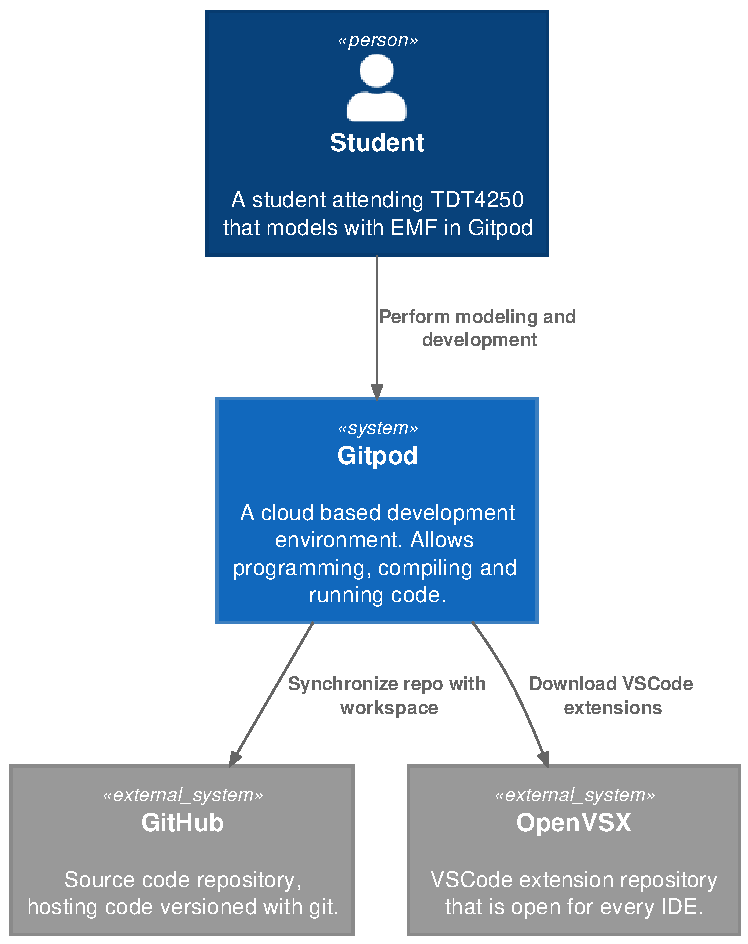
\includegraphics[width=\textwidth]{figures/plantuml/Gitpod_context.pdf}
  \caption[System context diagram for Gitpod]{A system context diagram for Gitpod. The extension will run inside the Gitpod service, used by a student to do modeling and developing. Gitpod uses git to synchronize code with GitHub. The extensions in Gitpod are downloaded from a service called OpenVSX.}\label{fig:gitpod-system-context}
\end{figure}

\begin{figure}[htbp]  % order of priority: h here, t top, b bottom, p page
  \centering
  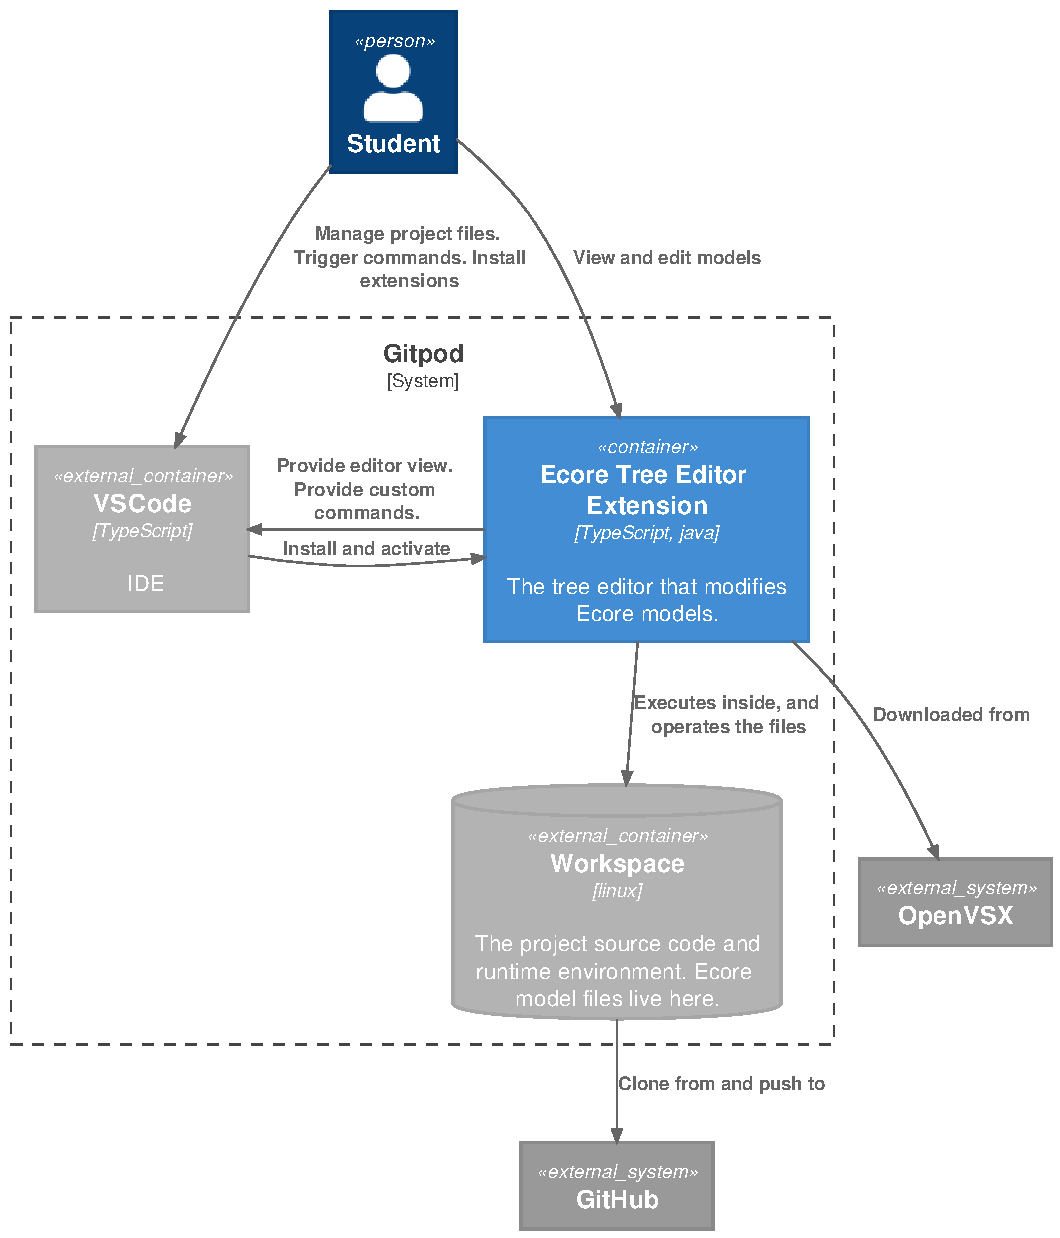
\includegraphics[width=\textwidth,height=\textheight,keepaspectratio]{figures/plantuml/Tree_Editor_Extension_container.pdf}
  \caption[Gitpod container diagram]{Container diagram for gitpod. The Gitpod system from \cref{fig:gitpod-system-context} is expanded to show its internal components. The \acrshort{IDE} used by Gitpod is \gls{Theia}.
  The student will interact with Theia, and install the Ecore Tree Editor Extension created from this thesis.
  This extension will also provide a user interface, which the student uses for modeling.
  This extension reads files from the Gitpod workspace, and uses the runtime provided by the workspace such as a Java Runtime Environment.}\label{fig:gitpod-container-diagram}
\end{figure}

\begin{figure}[htbp]  % order of priority: h here, t top, b bottom, p page
  \centering
  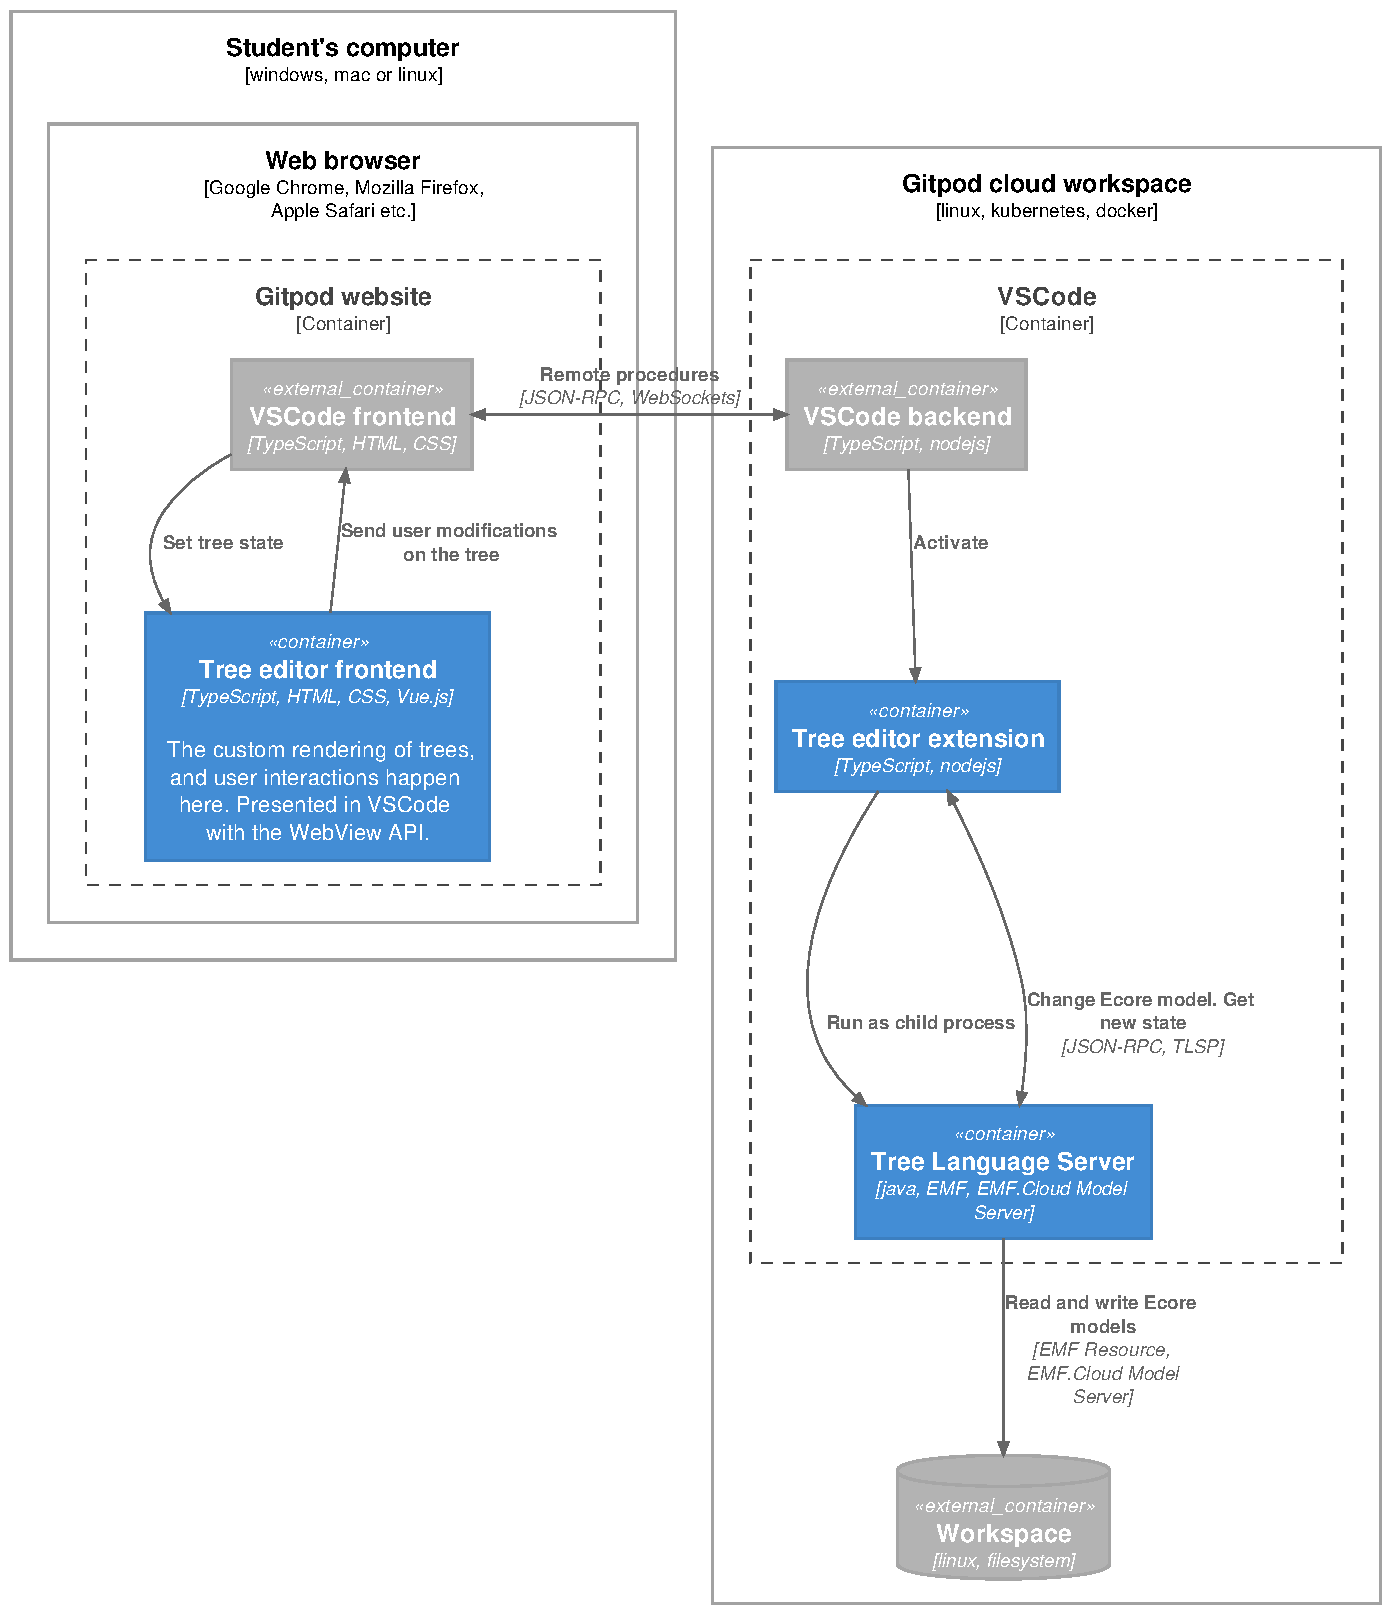
\includegraphics[width=\textwidth,height=\textheight,keepaspectratio]{figures/plantuml/Tree_Editor_Extension_deployment.pdf}
  \caption[Gitpod deployment diagram]{Deployment diagram of Gitpod. The student will use their computer to load the Gitpod website.
  The Gitpod service will start a computer in a cloud provider, to create a cloud workspace.
  The student only loads the Theia frontend and Tree editor frontend into their browser.
  Theia has a backend which runs inside the Workspace, and communicates to the frontend over WebSockets, using JSON-RPC\@.
  The Theia backend will activate the Tree editor extension, which in turn will start a Tree Language Server.
  This Tree Language Server runs java, and reuses the \acrshort{EMF} tooling.
  The Tree editor extension communicates to the Tree Language Server over a well defined protocol, where it asks to read model files, and execute commands to change the models.
  The Tree Language Server uses the Workspace to read and write \texttt{.ecore} files.}\label{fig:gitpod-deployment-diagram}
\end{figure}

\begin{figure}[htbp]  % order of priority: h here, t top, b bottom, p page
  \centering
  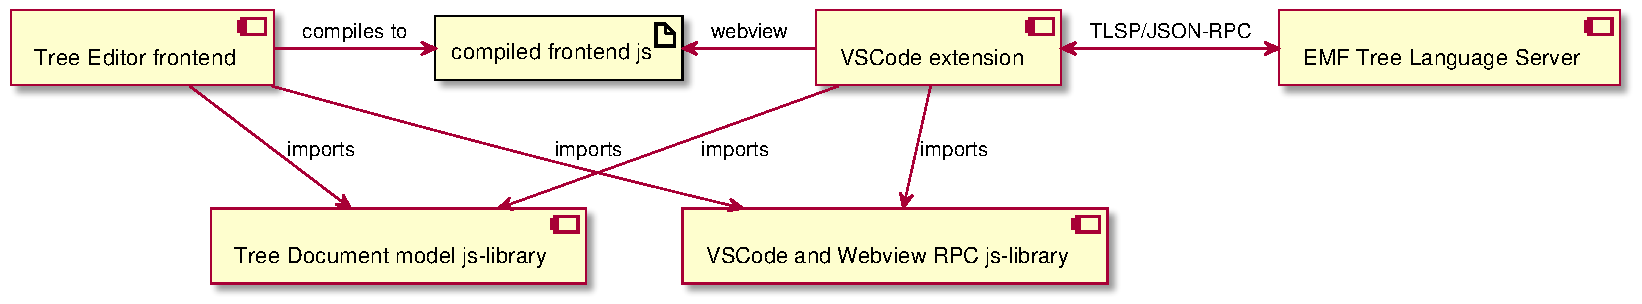
\includegraphics[width=\textwidth]{figures/plantuml/Tree_editor_components.pdf}
  \caption[Ecore Tree Editor component diagram]{Component diagram of the Ecore Tree Editor.
  The for the the extension is organized in 5 separate modules.
  The main module is the VSCode extension.
  This extension bundles the compiled frontend javascript artifact, and the compiled EMF Tree Language Server java jar-file.
  The Tree DOcument model js-library is the layer with the domain model for tree editors.
  It is used in both the frontend and the extension.
  }\label{fig:label4}
\end{figure}


\section{Software Artifact: Tree Editor Extension for Ecore in Visual Studio Code}
* Functioning viewer of any Ecore model in VSCode. Missing most features.
  * List of functional requirements implemented.
  * List of non-functional requirements implemented.
* Reuses java EMF code and EMF.Cloud ModelServer. No re-implementation of EMF logic.

* TLSP architecture. 3-component system (view, extension, server).

\section{Design Artifact: Tree Language Server Protocol}
% TODO

* TLSP protocol. JSON-RPC based with LSP Base, with a Tree Document Model data structure. Hierarchy schemas for optimistic-view drag-n-drop. Type and id based nodes. 

\section{Open Source Project: Measures Taken for Viability and Maintainability}
% TODO

* A project that may be viable and further developed.
  * Bundled IDE configuration: recommended extension, build tasks, run configurations. Reduces overhead for new developers.
  * NOT: CI/CD. Easily added later when needed. Overhead for 1-man project.
  * Build-scripts and npm/maven for building.
  * Readme-files for all components and modules.
  * Commonly used programming languages and (official) dependencies
  
